\section{Risultati Numerici}
\begin{frame}{Primi test sulla conservazione del volume}
  \begin{block}{Approssimazione del volume}
    Approssimiamo il volume, applicando la formula del punto medio
    composita a
    \[
    \int_{\Omega}(1-H(u(x)))dx\simeq\Delta x^3\sum_{i=1}^{|G_{\Delta x}|}(1-\tilde{H}(u(x)))
    \]
    con
    \[
    \tilde{H}(u)=
    \begin{cases}
      0 &u<-\varepsilon \\
      \frac{1}{2}+\frac{u}{2\varepsilon}+\frac{1}{2\pi}\sin{\frac{u\pi}{\varepsilon}}
        &-\varepsilon\leq u\leq\varepsilon \\
        1 &u>\varepsilon
    \end{cases}
    \]
 con $\varepsilon=1.5\Delta x$
  \end{block}
\end{frame}

\begin{frame}{Tabelle volume sfera}
\begin{table}[htb!]
\caption{Tabella per lo schema VPMCM. Evoluzione di una sfera.}
\label{tab:cp4-sc1-01}
\[
\begin{array}{*{6}{c}l}
    \toprule
    \text{time} &\text{nodi} &\Delta t &\text{iter}
    &\text{CPUs}&\text{VolE$_{\infty}$} &\text{VolE\ped{rel}} \\
     \midrule
     0.1        & 80         & 0.10    & 1          & 1,0s
     &1.1e^{-01} & 3.1e^{-03} \\ 
     0.2        &            &         & 2          & 3.7s
     &2.3e^{-01} & 6.9e^{-03} \\
     0.5        &            &         & 5          & 8,8s
     &7.5e^{-01} & 2.3e^{-02} \\ 
     1.0        &            &         & 10         & 21s
     &2.5e^{-00} & 7.6e^{-02} \\
    \midrule
     0.1        & 180        & 0.04    & 3          & 53s
     &1.1e^{-01} & 3.3e^{-03} \\ 
     0.2        &            &         & 5          & 91s
     &1.8e^{-01} & 5.3e^{-03} \\
     0.5        &            &         & 12         & 173s
     &2.9e^{-01} & 8.6e^{-03}  \\ 
     1.0        &            &         & 23         & 566s
     &2.3e^{-01} & 7.1e^{-03}  \\
    \bottomrule
\end{array}
\]
\end{table}
\end{frame}

\begin{frame}{\emph{Denoising} superfici geometriche}
  \begin{columns}[T]
    \begin{column}{4cm}
      \begin{block}{Rumore \emph{random}}
        Funzione che genera sfere di rumore random
        \begin{itemize}
        \item Numero di sfere
        \item Raggio delle sfere random in un range tra $[0$,raggioInput$]$ 
        \item Valore di rumore random tra $[0$,noiseInput$]$
        \end{itemize}
      \end{block}
    \end{column}
   \begin{column}{6cm}
     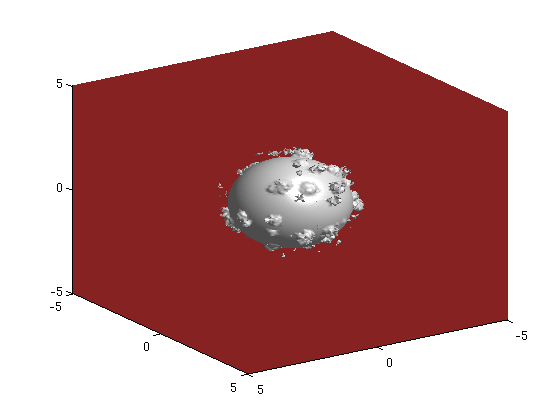
\includegraphics[width=1.0\textwidth]{noise/randNoise/mcm/sphere/sphere100r-0-00}
   \end{column}
  \end{columns}
\end{frame}

\begin{frame}{VPMCM vs MCM}
\begin{columns}[T]
  \begin{column}{5cm}
    \centering
    \only<1>{\animategraphics[autoplay,loop,width=1.0\textwidth,height=0.55\textheight]{0.8}{noise/randNoise/mcm/sphere/sphere100r-}{0}{5}}
    \end{column}
  \begin{column}[T]{5cm}
    \centering
    \only<1>{\animategraphics[autoplay,loop,width=1.0\textwidth,height=0.55\textheight]{0.8}{noise/randNoise/vpmcm/sphere/sphere100r-}{0}{5}}
    \end{column}
 \end{columns}
\begin{columns}[T]
  \begin{column}{5cm}
    \centering
    \only<2>{\animategraphics[autoplay,loop,width=1.0\textwidth,height=0.55\textheight]{0.8}{noise/randNoise/mcm/dumbbell/dumb100r-}{0}{4}}
    \end{column}
  \begin{column}[T]{5cm}
    \centering
    \only<2>{\animategraphics[autoplay,loop,width=1.0\textwidth,height=0.55\textheight]{0.8}{noise/randNoise/vpmcm/dumbbell/dumb100r-}{0}{4}}
    \end{column}
  \end{columns}
\end{frame}

\begin{frame}{\emph{Denoising} superfici geometriche}
 \begin{columns}[T]
   \begin{column}{4cm}
     \begin{block}{Rumore \emph{gaussiano}}
       Il rumore gaussiano è stato generato usando la funzione
       \emph{imnoise} di MATLAB, che simula il rumore con una distribuzione
       gaussiana.
     \end{block}
     \end{column}
   \begin{column}[T]{6cm}
     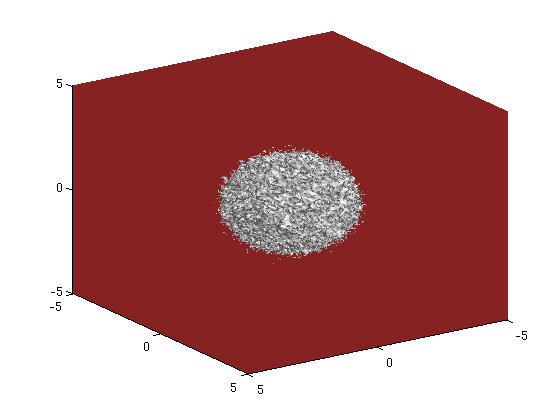
\includegraphics[width=1.0\textwidth]{noise/imnoise/mcm/sphere/sphere100i-0-00}
   \end{column}
 \end{columns}
\end{frame}

\begin{frame}{VPMCM vs MCM}
 \begin{columns}[T]
  \begin{column}{5cm}
    \centering
    \only<1>{\animategraphics[autoplay,loop,width=1.0\textwidth,height=0.55\textheight]{0.8}{noise/imnoise/mcm/sphere/sphere100i-}{0}{5}}
    \end{column}
  \begin{column}[T]{5cm}
    \centering
    \only<1>{\animategraphics[autoplay,loop,width=1.0\textwidth,height=0.55\textheight]{0.8}{noise/imnoise/vpmcm/sphere/sphere100i-}{0}{5}}
    \end{column}
 \end{columns}
\begin{columns}[T]
  \begin{column}{5cm}
    \centering
    \only<2>{\animategraphics[autoplay,loop,width=1.0\textwidth,height=0.55\textheight]{0.8}{noise/imnoise/mcm/dumbbell/dumb149i-}{0}{5}}
    \end{column}
  \begin{column}[T]{5cm}
    \centering
    \only<2>{\animategraphics[autoplay,loop,width=1.0\textwidth,height=0.55\textheight]{0.8}{noise/imnoise/vpmcm/dumbbell/dumb149i-}{0}{5}}
    \end{column}
  \end{columns}
\end{frame}

\begin{frame}{Immagine reale 3D}
 \begin{columns}[T]
    \begin{column}{4cm}
      \begin{block}{\emph{Gargolye}}
        \begin{itemize}
        \item Immagine ottenuta da uno scanner 3D
        \item La funzione levle-set non è regolare come le precedenti 
        \item Il metodo si comporta bene solo per poco iterazioni
        \item Abbiamo usato rumori piccoli
        \item Non sono molto evidenti le differenze con MCM
        \end{itemize}
      \end{block}
    \end{column}
   \begin{column}{6cm}
     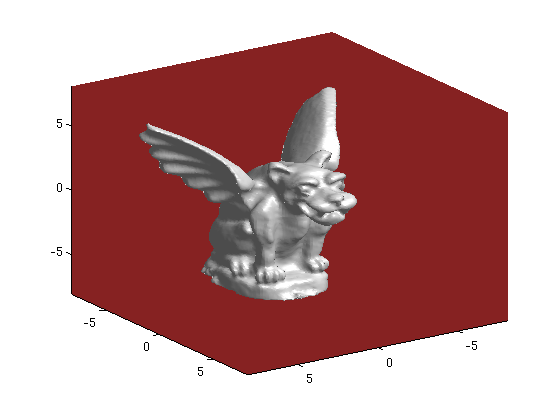
\includegraphics[width=1.0\textwidth]{smooth/mcm/gargolye/garg149-0-00}
   \end{column}
  \end{columns}
\end{frame}

\begin{frame}{Immagine reale 3D}
  \begin{columns}[T]
  \begin{column}{5cm}
    \centering
    \only<1->{\animategraphics[autoplay,loop,width=1.0\textwidth,height=0.55\textheight]{0.8}{noise/imnoise/vpmcm/gargolye/garg149i-}{0}{4}}
    \end{column}
  \begin{column}[T]{5cm}
    \centering
    \only<2>{\animategraphics[autoplay,loop,width=1.0\textwidth,height=0.55\textheight]{0.8}{noise/randNoise/vpmcm/gargolye/garg149r3-}{0}{3}}
    \end{column}
 \end{columns}
\end{frame}
